\chapter{Analýza pomocí metody 4ftMiner}
\label{ch:cleverminer}

Pomocí metody 4ftMiner, která je jednou z~metod procedury GUHA jsem provedla analýzu shrinků produktu. Tato metoda je implemnetovaná v~ knihovně \emph{Cleverminer} pro jazyk Python. Pracovala jsem pouze se vzorem dat jednoho měsíce a s~kategorií produktů \emph{Velmi čerstvé}, zastoupena 48, \% a \emph{Čerstvé}, zastoupena 52 \%. Princip metod, které se používají v~knihovně, a důležité pojmy týkající se GUHA procedur jsou popsány v~sekci \ref*{sec:Teorie:Guha}. 

Zkoumaný dataset se záznamy shrinků produktů jsem rozšířila o další sledované sloupce, které dávají do srovnání hodnotu shrinku a objem tržeb. Vytvořila jsem takto sloupce: podíl shrinku na celkových tržbách prodejny, podíl shrinku na týdenních tržbách shrinkovaného produktu na prodejně, podíl shrinku a tržeb v~kategorii úrovně 1.

Na základě zastoupení jednotlivých typů shrinků, kde prošlé a zkažené zboží zaujímá téměř 65 \% shrinků, se následující analýzy zaměřují pouze na tento typ, viz tab. \ref*{tab:shrinkyZastoupeni}.

\begin{table}[hbtp!]
    \begin{center}
            \captionsetup{justification=centering}
    \caption{Zastoupení vybraných shrinků ve zkoumaných datech \\(kategorie Čertvé a Velmi čerstvé).}
    \begin{tabular}{l r}
        Typ shrinku & Zastoupení v~kategoriích [\%]\\
        \midrule
        Prošlé a zkažené zboží & $64{,}97$ \\
        Potravinová banka & $23{,}72$ \\
         Poškození & $6{,}26$ \\
        Zvířecí útulky & $2{,}69$ \\
        Kompostéry &  $2{,}36$ \\
        \end{tabular}
    \label{tab:shrinkyZastoupeni}
\end{center}
\end{table}

Metoda pracuje pouze s~kategorickými hodnotami, proto bylo nutné kategorizovat sloupce s~hodnotou shrinku, s~množstvím shrinkovaných produktů a s~jednotlivými podíly. Na obrázcích \ref*{obr:nb:hist} až \ref{obr:nb:hist5} jsou zobrazené četnosti záznamů v~kategoriích.

\begin{figure}[h!]
    \centering
    \begin{minipage}[b]{.55\textwidth}
      \centering
      \captionsetup{justification=centering}

      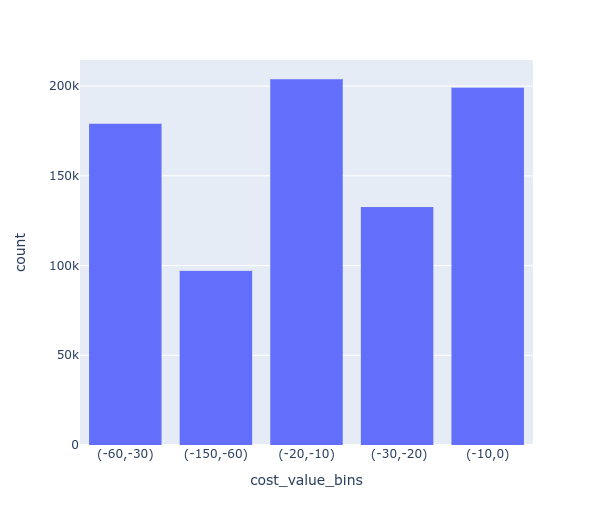
\includegraphics[width=\textwidth]{obrazky/grafy/histogram/newplot(2).png}
      \vspace*{-3em}
      \caption{Histogram pro hodnoty \\ velikosti shrinku v~peněžních jednotkách.}
      \label{obr:nb:hist}
    \end{minipage}%
    \hspace*{-2em}
    \begin{minipage}[b]{.55\textwidth}
        \centering
        \captionsetup{justification=centering}
        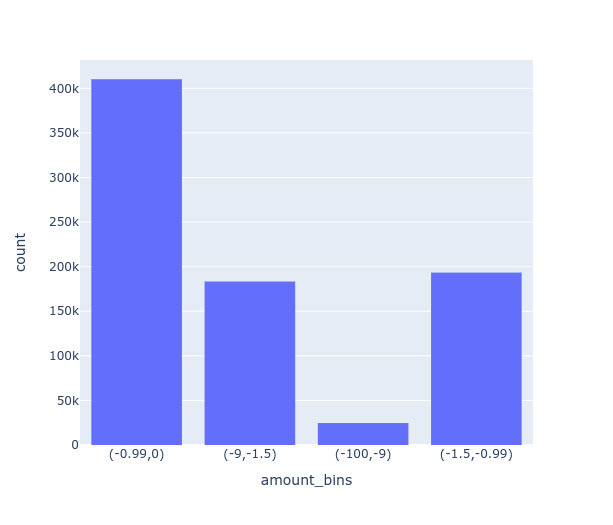
\includegraphics[width=\textwidth]{obrazky/grafy/histogram/newplot(1).png}
        \vspace*{-3em}
        \caption{Histogram pro hodnoty \\ objemu shrinku v~kusech.}
        \label{obr:nb:hist2}
    \end{minipage}
    \vspace*{-2em}

\end{figure}


\begin{figure}[h!]
    \centering
    \begin{minipage}[b]{.55\textwidth}
      \centering
      \captionsetup{justification=centering}

      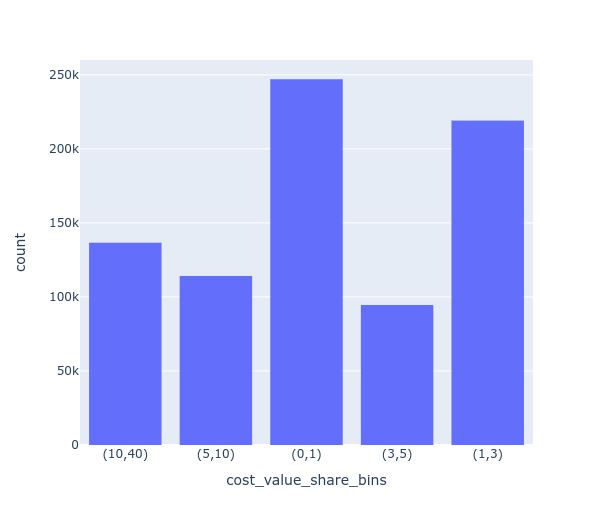
\includegraphics[width=\textwidth]{obrazky/grafy/histogram/newplot.png}
      \vspace*{-3em}
      \caption{Histogram podílu shrinku \\na tržbách shrinkovaného produktu.}
      \label{obr:nb:hist3}
    \end{minipage}%
    \hspace*{-2em}
    \begin{minipage}[b]{.55\textwidth}
        \centering
        \captionsetup{justification=centering}
  
        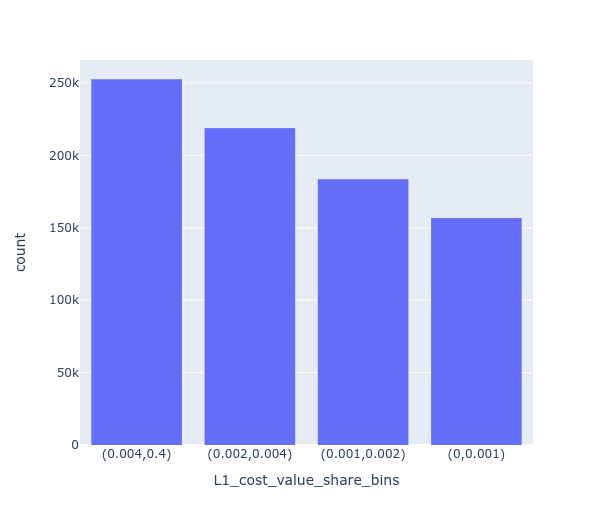
\includegraphics[width=\textwidth]{obrazky/grafy/histogram/newplot(3).png}
        \vspace*{-3em}
        \caption{Histogram podílu shrinku \\a tržeb v~kategorii úrovně 1.}
        \label{obr:nb:hist4}
    \end{minipage}     
       \vspace*{-1em}
\end{figure}

\begin{figure}[h!]
        \centering
        \captionsetup{justification=centering}
        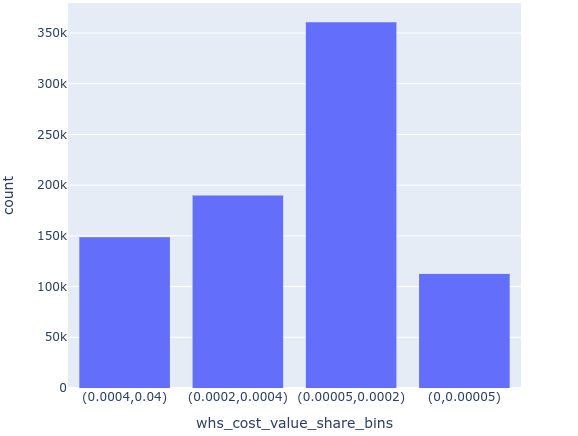
\includegraphics[width=0.55\textwidth]{obrazky/grafy/histogram/newplot(4).png}
        \caption{Histogram podílu shrinku \\na celkových tržbách prodejny.}
        \label{obr:nb:hist5}
        \vspace*{-1em}
\end{figure}

Pro první hypotézu je uvedeno volání funkce v~jazyce Python včetně předaných parametrů. Rovněž je v~tabulce uvedený celý výstup v~obdobném formátu jako je zobrazen na konzoli po ukončení běhu funkce. Dále už kódy, ani přesné výstupy uvedené nebudou, ale bude uveden pouze popis vstupů a komentář k~výstupům. 

\section{Hypotézy}

Před spuštěním metody bylo vždy třeba vznést hypotézu, která by mohla být pravdivá pro data týkající se shrinků. Tuto hypotézu pak přeformulovat do podoby asociačního pravidla, jehož pravdivost  na vstupních datech ověřuje metoda \emph{4ftMiner}. Tato metoda se předá jako parametr funkci \texttt{cleverminer}. Pravidlo se funkci zadává pomocí parametrů jako jednotlivé cedenty - antecedenty, sukcedenty, případně podmínky. Více o principu metody je ovedeno v~teoretické části práce.

\vspace*{1em}

\textbf{Hypotéza č. 1: Objem prošlého zboží je závislý na typu promoakce a dni v~týdnu}

Ve zkoumaných datech je zboží bez promoakce zastoupeno $58{,}2$ \%, zboží týden po evidované promoakci $23{,}2$ a zboží v~promoakci $18{,}6$ procentem. 

Asociační pravidlo má tvar:
\begin{equation}
    \varphi_{\mbox{\,\footnotesize Den v~týdnu}} \land \varphi_{\,\mbox{\footnotesize Typ promoakce}} \Rightarrow \psi_{\mbox{\,\footnotesize Množství}}
\end{equation}

V ukázce kódu \ref*{code:cleverminerH1} jsou uvedené parametry pro spuštění metody. Konfidence byla zvolena 80 \%. Výsledky běhu jsou uvedené v~tabulce \ref*{tab:H1vysl}. Z této tabulky lze vyčíst, že pro vybrané dny v~týdnu -- pondělí, úterý, středa, čtvrtek a neděle, tj. nikoli pro pátek a sobotu -- a pro produkty, které byly v~den záznamu týden po promoakci platí, že 80 \% těchto záznamů bylo v~množství do jednoho kusu. To znamená, že se jedná o produkty, které jsou vážené. Jejich přepočet na kusovou jendotku tedy může být menší než jeden celý kus. Podle dalšího zkoumání dat jsem zjistila, že se jedná především o kategorii \emph{Masné výrobky} ze třetí úrovně hierarchie.


\begin{lstlisting}[language=Python, style=mystyle, label={code:cleverminerH1}, caption={Hypotéza č. 1, funkce \texttt{cleverminer}.}]
cleverminer(df = data,
            proc = "4ftMiner", 
            quantifiers = {"conf":0.8, "Base":1000},
            ante = {
                    "attributes":
                    [
                        {
                            "name":"weekday", 
                            "type":"seq", 
                            "minlen":1, "maxlen":3
                        },
                        {
                            "name":"promo", 
                            "type":"sec", 
                            "minlen":1, "maxlen":1
                        }
                    ], 
                    "minlen":2, "maxlen":2, "type":"con"
                    },
            succ = {
                    "attributes":
                    [
                        {
                            "name":"amount_bins", 
                            "type":"subset", 
                            "minlen":1, "maxlen":1
                        }
                    ], 
                    "minlen":1, "maxlen":1, "type":"con"
                    }
            )
    \end{lstlisting}

    \begin{table}[h!]
        \begin{center}
                \captionsetup{justification=centering}
        \caption{Výstup funkce \texttt{cleverminer} pro hypotézu 1.}
        \begin{tabular}{rrrp{7.5cm}}
            Základ ($a$) & Konfidence & AAD & AP [\%]\\
            \midrule
19765 & 0.821 & $+0.623$ & weekday(0) $\land$ promo(after\_promo) $\Rightarrow$ amount\_bins((-0.99,0)) \\
39271 & 0.820 & +0.622 & weekday(0, 1)  $\land$ promo(after\_promo) $\Rightarrow$ amount\_bins((-0.99,0)) \\
63920 & 0.815 & +0.613 & weekday(0, 1, 2)  $\land$ promo(after\_promo) $\Rightarrow$ amount\_bins((-0.99,0)) \\
19506 & 0.820 & +0.621 & weekday(1)  $\land$ promo(after\_promo) $\Rightarrow$ amount\_bins((-0.99,0)) \\
44155 & 0.813 & +0.608 & weekday(1, 2)  $\land$ promo(after\_promo) $\Rightarrow$ amount\_bins((-0.99,0)) \\
68666 & 0.810 & +0.603 & weekday(1, 2, 3)  $\land$ promo(after\_promo) $\Rightarrow$ amount\_bins((-0.99,0)) \\
24649 & 0.808 & +0.598 & weekday(2)  $\land$ promo(after\_promo) $\Rightarrow$ amount\_bins((-0.99,0)) \\
49160 & 0.806 & +0.595 & weekday(2, 3)  $\land$ promo(after\_promo) $\Rightarrow$ amount\_bins((-0.99,0)) \\
24511 & 0.805 & +0.593 &weekday(3) $\land$ promo(after\_promo) $\Rightarrow$ amount\_bins((-0.99,0)) \\
18864 & 0.813 & +0.608 &weekday(6)  $\land$ promo(after\_promo) $\Rightarrow$ amount\_bins((-0.99,0)) \\
    \end{tabular}
\label{tab:H1vysl}
\end{center}
\end{table}

\vspace*{1em}

\textbf{Hypotéza č. 2: Kategorie shrinkovaného zboži je závislá na typu promoakce a dni v~týdnu}

Asociační pravidlo má tvar:
\begin{equation}
    \varphi_{\mbox{\,\footnotesize Den v~týdnu}} \land \varphi_{\,\mbox{\,\footnotesize Typ promoakce}} \Rightarrow \psi_{\mbox{\,\footnotesize Hierarchie3}} \lor \psi_{\mbox{\,\footnotesize Hierarchie4}},
\end{equation}
kde označením Hierarchie3 jsou myšleny kategorie na třetí úrovni produktové hierarchie, obdobně pro pojem Hierarchie4.

Parametry předané funkci jsou podobné jako u předchozí hypotézy. Ze záznamů, které se byly porvedeny v~pondělí, úterý nebo neděli a týkaly se produktů, které byly v~rozmezí  jednoho týdne po promoakci, bylo více než 75 \% z~kategorie Masné výrobky -- pultový prodej ze čtvrté úrovně produktové hierarchie. Pokud je vynechána ze vstupních dat tato kategorie, pak maximální konfidence 31 \% byla dosažena pro kategorii Slaného pečivo v~záznamech, které byly provedeny v~sobotu a týkaly se produktů zcela mimo promoakci. Jiné významné závislosti podle dat nebyly nalezeny.

\vspace*{1em}

\textbf{Hypotéza č. 3: Na některých lokalitách vyhazují často stejné produkty}

Asociační pravidlo má tvar:
\begin{equation}
    \varphi_{\mbox{\,\footnotesize Typ prodejny}} \land \varphi_{\,\mbox{\footnotesize Okres}} \Rightarrow \psi_{\mbox{\,\footnotesize Množství}}
\end{equation}

60 \% záznamů týkajících se okresů Jindřichův Hradec, Ústí nad Labem, Písek nebo Strakonice tvoří shrinky z~kategorie \emph{Masné výrobky}. Pro záznamy z~okresu Kladno, které jsou zároveň evidovány velkými prodejnami kategorie Masné výrobky byla zastoupena až téměř 70 \%. Necelými 70 \% je tato kategorie zastoupená také v~záznamech v~malých prodejnách v~okrese Praha-východ.

Pokud úplně vynecháme kategorie Masné produkty ze vstupních dat, pak se nejčastěji ve výsledcích objevovala kategorie \emph{Pečivo}. Pro záznamy z~velkých prodejen v~okrese Pardubice nebo Plzeň-město Pečivo zaujímalo přes 60 \% těchto záznamů. Nad 50 \% záznamů pro okresy Bruntál, Olomouuc, Příbram nebo Uherské Hradiště. 50 \% záznamů náleželo kategroii Pečivo také v~záznamech z~malých prodejen v~okrese Klatovy, Náchod nebo Přerov.

Po vynechání kategorie Pečivo již dostáváme maximální konfidenci 33 \%, a to pro kategorii Zelenina ve zbylých záznamech z~okresu Ostrava-město, Kroměříž, Hradec Králové nebo Karvinná.

\vspace*{1em}

% \textbf{Hypotéza č. 3: Na některých v~některých lokalitách mají často zaznamenané shrinky s~malou hondotou vzhledem k~tržbám prodejny.}

% Tvar asociačního pravidla:
% \begin{equation}
%     \varphi_{\mbox{\,\footnotesize Okres}} \land \Rightarrow \psi_{\mbox{\,\footnotesize Podíl na prodejně}}
% \end{equation}

% Ve všech záznamech pro okres Chrudim zaujímalo 57 \% z~nich 

\textbf{Hypotéza č. 4: Některé produkty se vyhazují častěji než jiné, ale v~malém množství.}

Asociační pravidlo pro úroveň produktové hierarchie 3 má následující tvar. Pro úroveň 4 je tvar AP analogický.
\begin{equation}
    \varphi_{\mbox{\,\footnotesize Hierarchie3}} \Rightarrow \psi_{\mbox{\,\footnotesize Množství}}
\end{equation}

% Nejprve je vhodné ukázat kolik činí četnost vybraných kategorií v~datech.
Kategorie Masné produkty byla zaznamenána téměř 300 tisíckrát, a v~94 procentech se jednalo o množství odpovídající do jednoho balení. Podkategorie Masné produkty -- pultový prodej má 99 \% svých záznamů do jednoho kusu.
Pokud se vyhazují čerstvé ryby, tak v~94 \% jeich záznamů je to množství do jednoho kusů. Kategorie Drobné občerstvení %Tapas
 se vyhazuje v~89 \% po jednom kusu (obvykle se jedná o sendviče a bagety)
Kategorie Vejce se vyhazuje v~82 \% po jednom kusu balení
Kategorie Pečivo se vyhazuje v~56 \% v~počtu kusů do 10~kusů v~až 94~tis. záznamech.
Kategorie Jádroviny\footnote{Jádroviny jsou druh ovoce, patří sem např. jablka a hrušky.} se vyhazuje 74 \% případech svých záznamů (14 000 záznamů) v~množství do jednoho kusu. I zde se jedná přepočet váženého množství na kusy.

\vspace*{1em}

\textbf{Hypotéza č. 5: Některé vyhazované kategorie produktů jsou výrazně nákladnější.}

Asociační pravidlo má tvar:
\begin{equation}
    \varphi_{\mbox{\,\footnotesize Hierarchie4}} \Rightarrow \psi_{\mbox{\,\footnotesize Shrink}}
\end{equation}

Pokud se vyhazují čerstvé ryby, tak v~téměř 80 \% případech záznamů jsou ztracené náklady jednoho záznamu vyšší, a to v~rozmezí 60-150 pěněžních jednotek.
Pokud se vyhazuje kategorie Červené maso, tak z~téměř 60 \% je ztráta v~rozsahu 60-150 jendotek.
Kategorie Chlazený pultový prodej, která obsahuje např. čerstvé chlebíčky, saláty a pochutiny, se v~50 \% vyhazuje v~hodnotě do 10 pěněžních jendotek. Jedná se tedy o nižší částky, které jsou ale časté. Záznamů této kategorie bylo evidováno $12{,}5$ tisíc.
Cukrářské výrobky byly evidovány v~1835 záznamech. 66 \% těchto záznamů mělo hodnotu mezi 10 a 20 pěněžními jednotkami.

\vspace*{1em}

\textbf{Hypotéza č. 6: Shrink některých kategorií je v~porovnání s~tržbami těchto produktů na stejné prodejně velký.}

Asociační pravidlo má tvar:
\begin{equation}
    \varphi_{\mbox{\,\footnotesize Hierarchie4}} \Rightarrow \psi_{\mbox{\,\footnotesize Podíl shrinku na svých tržbách}}
\end{equation}

Nejedná se o porovnání s~celkovými tržbami prodejny, ale pouze o týdenní tržbu těch produktů, které měly zaznamenaný v~daném týdnu shrink.
Kategorie Drobné občerstvení má podíl shrinku na svých tžbách v~84 \% ze zaznamenaných případů mezi 10-40 \%.
Cukrářské výrobky  mají podíl shrinku v~74 \% zaznamenaných případech také mezi 10-40 \%.
Banány mají podíl shrinku na tržbách banánů v daném týdnu v~80 \% ze svých zaznamenaných případech do 1 \%. To znamená, že se jedná o malou část svého prodeje,
Více než 30 tis. záznamůs se týká kategorie Citrusů a kategorie Jádrovin. Přibližně 65 \% těchto záznamů je podíl shrinku do 1 \% na tržbách těchto produktů.

Dále pro tuto hypotézu bylo oběřováno podmíněné asociační pravidlo:
\begin{equation}
    \varphi_{\mbox{\,\footnotesize Hierarchie3}} \Rightarrow \psi_{\mbox{\,\footnotesize Podíl shrinku na svých tržbách}} | \chi_{\mbox{\,\footnotesize Shrink}}
\end{equation} 

Následující tvrzení platí s více než 83\% konfidencí.
Pokud mezi produkty, kterým byl zaznamenán dražší shrink, tj. 30-60 pěněžních jednotek, jsou produkty z kategorie Jogurty, tak podíl shrinku na jejich tržbách je mezi 10-40 \%. Totéž tvrzení platí i pro kategorii Drobného občerstvení.
Pokud mezi produkty, kterým byl zaznamenán levný shrink, tj. do 10 peněžních jednotek, je ovoce, tak jejich share shrinku na tržbách je do 1 \%. To samé platí o pro kategorii Kořenová zelenina.

\vspace*{1em}

\textbf{Hypotéza č. 7: Kategorie má vliv na zastoupení shrinku na celkových tržbách prodejny v~dané kategorii úrovně 1.}

S pravděpodobností vyšší než 50 \% se toto tvrzení potvrdilo pouze u kategorie Bylinky z~úrovně 4, kdy shrink této kategorie tvoří 0.002 \% až 0.005 \% tržeb na prodejnách v kategorii Velmi čerstvé v prvním levelu produktové hierarchie.

\vspace*{1em}

\textbf{Hypotéza č. 8: Den v~týdnu nebo čtvrtina měsíce mají vliv na záznamy.}

Asociační pravidlo je následovné:
\begin{equation}
    \varphi_{\mbox{\,\footnotesize }} \Rightarrow \psi_{\mbox{\,\footnotesize Podíl shrinku na svých tržbách}} | \chi_{\mbox{\,\footnotesize Shrink}}
\end{equation} 

Záznamy uskutečněné ve středu, čtvrtek a pátek v~poslední čtvrtině měsíce, takových je přes 100 tisíc, se ze 67\% konfidencí týkají malých prodejen.